\begin{figure}[H]
  \centering
    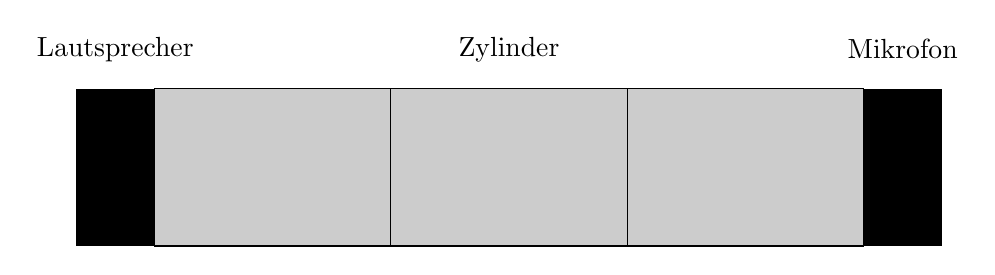
\begin{tikzpicture}
      \fill (0,0)--(0,2)--(1,2)--(1,0)--cycle;
      \node at (0.5,2.5) {Lautsprecher};

      \filldraw[fill=white!80!black] (1,0)--(4,0)--(4,2)--(1,2)--cycle;
      \filldraw[fill=white!80!black] (4,0)--(7,0)--(7,2)--(4,2)--cycle;
      \filldraw[fill=white!80!black] (7,0)--(10,0)--(10,2)--(7,2)--cycle;
      \node at (5.5,2.5) {Zylinder};

      \fill (10,0)--(10,2)--(11,2)--(11,0)--cycle;
      \node at (10.5,2.5) {Mikrofon};
    \end{tikzpicture}
  \caption{Skizze des Zylinderaufbaus}
  \label{fig:aufbau_zylinder}
\end{figure}

\begin{figure}[H]
  \centering
    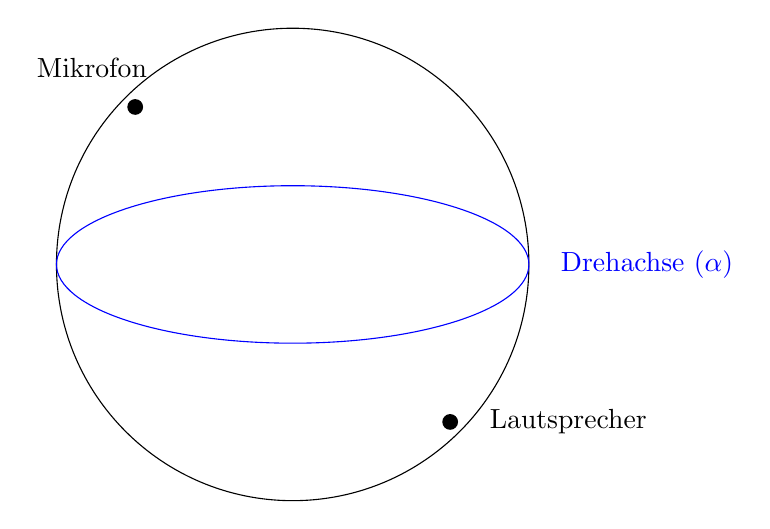
\begin{tikzpicture}
      \draw (0,0)circle(3);
      \draw[blue] (0,0)ellipse(3 and 1);
      \node[blue] at (4.5,0) {Drehachse ($\alpha$)};
      \fill (2,-2)circle(0.1);
      \node at (3.5,-2) {Lautsprecher};
      \fill (-2,2)circle(0.1);
      \node at (-2.55,2.5){Mikrofon};
    \end{tikzpicture}
  \caption{Skizze des Kugelaufbaus}
  \label{fig:aufbau_kugel}
\end{figure}

\begin{figure}[H]
  \centering
    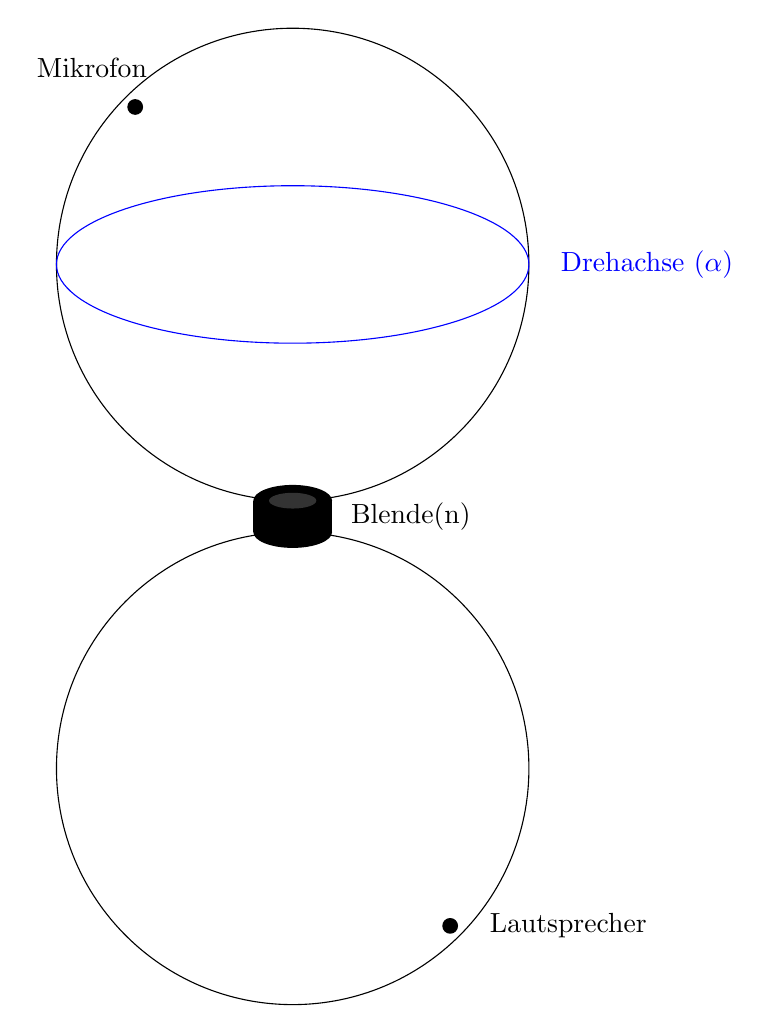
\begin{tikzpicture}
      \draw (0,0)circle(3);
      \fill (-0.5,-3)--(0.5,-3)--(0.5,-3.4)--(-0.5,-3.4)--cycle;
      \fill (0,-3.4)ellipse(0.5 and 0.2);
      \fill (0,-3)ellipse(0.5 and 0.2);
      \fill[black!80!white] (0,-3)ellipse(0.3 and 0.1);
      \node at (1.5,-3.2) {Blende(n)};
      \draw (0,-6.4)circle(3);
      \draw[blue] (0,0)ellipse(3 and 1);
      \node[blue] at (4.5,0) {Drehachse ($\alpha$)};
      \fill (2,-8.4)circle(0.1);
      \node at (3.5,-8.4) {Lautsprecher};
      \fill (-2,2)circle(0.1);
      \node at (-2.55,2.5){Mikrofon};
    \end{tikzpicture}
  \caption{Skizze des gekoppelten Kugelaufbaus}
  \label{fig:aufbau_kugel_2}
\end{figure}
